\documentclass[a4paper,12pt]{article}
\usepackage[latin1]{inputenc}
\usepackage[pdftex]{color,graphicx}
\usepackage[hypertexnames=false]{hyperref} 
\usepackage[german,ngerman]{babel}
\usepackage{fancyhdr}
\usepackage{amssymb}
\usepackage{background}
\usepackage{amsmath}
\usepackage[rflt]{floatflt}
\usepackage{tabularx}
\usepackage{ausarbeitung}
\usepackage{listings}
\usepackage{color}
\usepackage[T1]{fontenc}
\usepackage{mathpazo}
\usepackage{lmodern}

\newcommand{\pfile}[1]{{\bfseries \ttfamily #1}}

%% Diese Farben werden f�r den Quelltext verwendet
\definecolor{srcblue}{rgb}{0,0,0.5}
\definecolor{srcgray}{rgb}{0.5,0.5,0.5}
\definecolor{srcred}{rgb}{0.5,0,0}

\definecolor{mygreen}{rgb}{0,0.6,0}
\definecolor{mygray}{rgb}{0.5,0.5,0.5}


\lstdefinelanguage{JavaScript}{
  keywords={typeof, new, true, false, catch, function, return, null, catch, switch, var, if, in, while, do, else, case, break},
  ndkeywords={class, export, boolean, throw, implements, import, this},
  identifierstyle=\color{black},
  sensitive=false,
  comment=[l]{//},
  morecomment=[s]{/*}{*/},
  morestring=[b]',
  morestring=[b]"
}

\lstset{basicstyle=\scriptsize, numbers=left, numberstyle=\tiny\color{mygray}, numbersep=5pt, captionpos=b,  basicstyle=\footnotesize\ttfamily,
  keywordstyle=\color{blue}\bfseries, 
  ndkeywordstyle=\color{darkgray}\bfseries,
  commentstyle=\itshape\color{green!40!black},
  stringstyle=\color{srcblue},breaklines=true}



\renewcommand{\lstlistingname}{Quellcode}% Listing -> Algorithm
\renewcommand{\lstlistlistingname}{\lstlistingname verzeichnis}% List of Listings

%% Diese Zeile unbedingt stehen lassen und anpassen - sie enth�lt Autor und Titel der Ausarbeitung
\mywork{David Bujok}{Thema der Arbeit}

\begin{document}
\SetBgContents{}
	%% Bei Diplomarbeiten folgende Zeile nutzen
	\mybachelortitle{Dipl.-Wirt.Inform. Claus Alexander Usener}
	%% Bei Bachelorarbeiten diese Zeile auskommentieren
	%%\mybachelortitle{(ggf. Name des Betreuers)}
	%% Bei Seminararbeiten diese Zeile auskommentieren
	%%\myseminartitle{Titel des Seminars}{(ggf. Name des Betreuers)}

  %% Inhaltsverzeichnis
  %% frontmatter setzt die Seitenzahlen auf i, ii, ...
  \frontmatter

	%% Generiert automatisch aus den Sektionsbefehlen ein Inhaltsverzeichnis  
  \tableofcontents
  \newpage
%	\lstlistoflistings
%	\newpage
%	\listoffigures
%   \newpage

	%% das Mainmatter sorgt f�r die Nutzung arabischer Seitenzahlen
	\mainmatter
	
\section{Einleitung}
\label{sec:einleitung}

Bei Moodle handelt es sich um ein Softwarepaket, welches einen  konstruktivistischen Lehr- und Lernansatz unterst�tzt. \cite{moo15a}
 Weltweit in 231 L�ndern �ber 53.000 Seiten registriert \cite{moo15a}
 
 Moodle ist international die am weitesten verbreitete Lernplattform \cite{hei15}.
 
%Moodle ist eine frei verf�gbare Open Source Software. Dies bedeutet, dass sie frei erhaeltlich ist. Au�erdem bietet Sie die M�glichkeit der individuellen Anpassung an spezifische Anwendungssituationen \cite{moo15a}.

Die Westf�lische Wilhelms-Universit�t M�nster stellt zur Verbesserung des Lehrbetriebs eine Moodledistribution unter dem Namen Learnweb zur Verf�gung.

F�r die Vorlesung \textit{Informatik I} wurde bereits ein Moodlemodul implementiert, welches die M�glichkeit  bietet ????

Die Arbeit wird durch ein Grundlagenkapitel (Kapitel \ref{sec:grundlagen}) eingeleitet, in die zentralen Ideen von E-Assessment vorgestellt und 
die wesentlichen Merkmale der Lernplattform Moodle hervorgehoben werden. Bei der Vorstellung von Moodle wird auf die Pluginstruktur der Plattform eingegangen. 

Im darauffolgenden Kapitel (Kapitel \ref{sec:dsbuilder}) wird das Modul EASy-DSBuilder vorgestellt. Hierbei wird auf die Funktionalit�t aus Benutzersicht und auf die Struktur aus technischer Sicht eingegangen.


\section{E-Assessment}


\subsection{Einleitung}
In der Hochschullehre nehmen Leistungs�berpr�fungen einen integralen Bestandteil in Lehr- und Lernprozessen ein. Ein Augenmerk liegt hierbei auf der Identifizierung und Bewertung individueller Lernfortschritte \cite[S. 23 f.]{Kuchen2010}. Darunter wird insbesondere das Pr�fen und Bewerten einzelner �bungen als Teil einer p�dagogischen Handlungseinheit verstanden. Dabei k�nnen die verschiedenen �bungsphasen und -iterationen unterschiedliche L�ngen haben und inhaltliche Abh�ngigkeiten haben \cite[S. 25]{Kuchen2010}. Abbildung \ref{fig:Uebungsbetrieb} zeigt den Lehr-Lern-Prozess eines �bungsbetriebs.

\begin{figure}[htbp] 
  \centering
     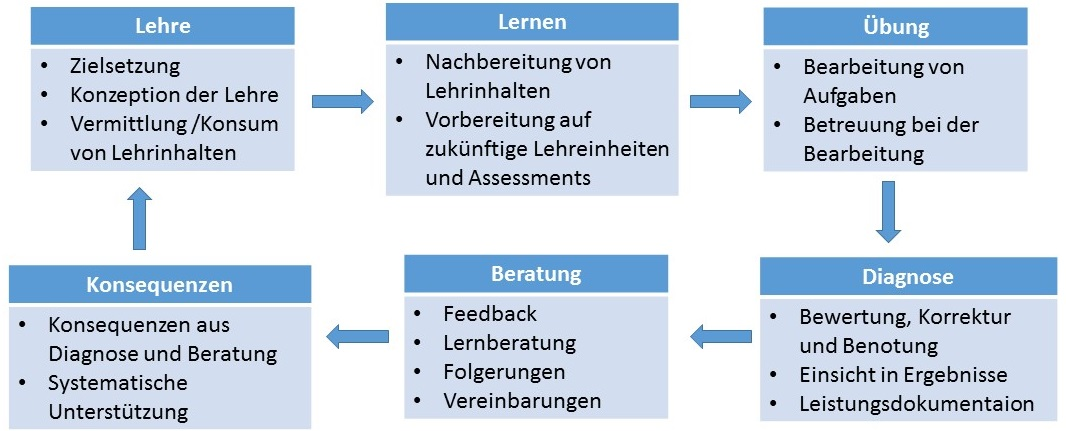
\includegraphics[width=0.9\textwidth]{graphics/Uebungsbetrieb.jpg}
  \caption{Iterative Lehr-Lern-Prozesse eines �bungsbetriebs}
  \label{fig:Uebungsbetrieb}
\end{figure} 

Im Regelfall beginnt ein �bungszyklus mit der Phase der Lehre. In dieser Phase vermittelt der Lehrende dem Studierenden die entsprechenden Inhalte. Anschlie�end hat der Studierende in der Lernphase die M�glichkeit das vermittelte Wissen im Selbststudium zu vertiefen. In einer darauf folgenden �bung kann der Studierende sein theoretisches Wissen anhand geeigneter praktischer �bungen ausprobieren und festigen. Im Anschluss folgt die Diagnose der �bung, welche Korrektur und Benotung beinhaltet. Dies geschieht im Regelfall durch DozentInnen oder TutorInnen, kann aber auch durch KommilitonInnen erfolgen (Peer Review). Es sollte ein Feedback �ber die erbrachte Leistung und Ratschl�ge folgen. Optional kann aus den Ratschl�gen eine Leistungsvereinbarung abgeleitet werden \cite[S. 25 f.]{Kuchen2010}.

Auf Grund des Bologna-Prozesses, Sparma�nahmen, Diskussionen �ber die Verwendung von Studiengeb�hren und steigende Studierendenzahlen wird im Bereich der �bungsangebote der Einsatz von E-Assessments vermehrt in Betracht gezogen \cite[S. 9]{kortemeyer2010}. 
Unter e-Assessment versteht man das Spektrum der auf den neuen (elektronischen) IKT basierenden Verfahren der lehrzielbezogenen Bestimmung, Beurteilung, Bewertung, Dokumentation und R�ckmeldung der jeweiligen Lernvoraussetzungen, des aktuellen Lernstandes oder der erreichten Lernergebnisse/ -leistungen vor, w�hrend (?Assessment f�r das Lernen?) oder nach Abschluss (?Assessment des Lernens?) einer spezifischen Lehr-Lernperiode \cite[S. 6]{Bloh2006}. E-Assessment-Systeme k�nnen des Weiteren Nutzen f�r Lehrende und Lernende bieten. Cook und Jenkins identifizierten neuen Vorteile. Bei den Wichtigsten handelt es sich um die M�glichkeiten des direkten Feedbacks und der sofortigen und objektiven Benotung.  Au�erdem bieten E-Assessment-Systeme einfache Skalierbarkeit und Wiederverwendbarkeit \cite[S. 3]{Cook2010}. E-Assessments k�nnen hinsichtlich ihrer Hauptaufgabe in drei Typen unterteilt werden \cite[S. 8]{Cook2010}:
\begin{itemize}
\item \textbf{Diagnostische Assessments} finden normalerweise zu beginn einer Lehrveranstaltung statt um m�gliche Wissensl�cken bei Teilnehmern aufzudecken und gegebenenfalls ein Nachbesserungsangebot zu schaffen. 
\item \textbf{Formative Assessments} erm�glicht Studierenden und Lehrenden einen �berblick �ber den aktuellen Lernstand zu erhalten. E-Assessment erm�glicht Studierenden weiterhin ein direktes Feedback.
\item \textbf{Summative Assessments} bieten eine Bewertungsgrundlage �ber den Lernfortschritt eines Studierenden. Bei diesem Typen steht im Gegensatz des Feedbacks die Notengebung im Vordergrund.
\end{itemize}

Leistung�berpr�fungen sind ein integraler Bestandteil der Lehr- und Lernprozesse. \cite{Kuchen2010}. 

W�chentliche �bungszettel --> theoretisch erlerntes Wissen durch Bearbeitung geeigneter Aufgaben reflektieren und verinnerlichen S.24



\subsection{Das E-Assessment-System EASy der WWU M�nster}
\subsubsection{Aufbau eines Plugins}
\label{sec:aufbauPlugin}

F�r jedes Plugin in Moodle muss eine bestimmte Datenstruktur implementiert werden. Diese besteht aus separaten Unterverzeichnissen und verpflichtenden Dateien. Des weiteren haben Entwickler die M�glichkeit weitere Dateien selbst zu gestalten. 

\paragraph{/backup}

\paragraph{/db}
\begin{itemize} 
	\item \textbf{/access.php}
	\item \textbf{/install.xml}
	\item \textbf{log.php}
	\item \textbf{upgrade.php}
\end{itemize}
\paragraph{/lang}

\paragraph{/}
\section{Vorstellung des Moodlemoduls EASy-DSBuilder}
\label{sec:dsbuilder}
Der EASy-DSBuilder ist ein E-Assessent Tool, welches der Evaluation grundlegender Konzepte �ber Operationen (z.B. Suchen, Einf�gen, und Entfernen) innerhalb der Datenstruktur \textit{Bin�rbaum} dient \cite{Usener2014}.
Das Tool wurde speziell f�r die Lernplattform Moodle implementiert. 

Diese Kapitel wird das Tool EASy-DSBuilder vorstellen. Hierbei wird zu erst in Kapitel \ref{sec:funktionalitaet} auf die Funktionalit�t aus Benutzersicht eingegangen. Anschlie�end erfolgt eine Erl�uterung der technischen Umsetzung (Kapitel \ref{sec:technologien}).

\subsection{Funktionalit�t aus Benutzersicht}
\label{sec:funktionalitaet}

Im folgenden Kapitel wird die Funktionalit�t des Moodlemodul EASy-DSBuilder vorgestellt. Hierbei wird auf die beiden Sichten Studierender und Lehrender eingegangen.

\paragraph{Lehrender} \hfill \\
Der Lehrende hat zwei grundlegende Aufgaben. Zum Einen ist er daf�r verantwortlich, dass eine Aufgabe erstellt wird, zum Anderen hat er die M�glichkeit, die Abgaben einzusehen, um sie beispielsweise zu bewerten oder Indikatoren zur Verbesserung der Lehre zu finden \cite{Usener2014}. Wird eine neue Aufgabe erstellt, hat der Lehrende die M�glichkeit allgemeine Informationen wie den \textit{Titel}, die \textit{Beschreibung} und das \textit{F�lligkeitsdatum} anzugeben. Unter \textit{Source Files} kann der Lehrende �ber Drag-and-Drop seine eigene Implementierung einer Datenstruktur zu dem Moodlemodul hinzuf�gen. Hierzu muss er einen Wrapper auf Basis des Interfaces \textit{DataStructureWrapperInterface<K extends Comparable<K>, D>} implementieren (vergl. Anhang, Quellcode \ref{code:wrapper}). Diese Wrapperklasse muss anschlie�end vom Lehrenden als Hauptklasse eingestellt werden. Auf die Funktionalit�t der Wrapperklasse aus technischer Sicht wird im Kapitel \ref{sec:technWebService} n�her eingegangen. Des weiteren kann der Lehrende eine Feedback aktivieren. Die genau Funktionalit�t des Feedbacks wird im Abschnitt �ber die Funktionalit�t aus Sicht des Studierenden erl�utert.  

\paragraph{Studierender} \hfill \\
Der Studierende verf�gt �ber zwei Ansichten. Zum einen gibt es die �bersichtsansicht, zum anderen die Bearbeitungsansicht.
Nachdem der Studierende sich in das Modul eingew�hlt hat, ist die �bersichtsansicht �ber den bisherigen Verlauf des Assessments zu sehen. In dieser �bersicht ist der Abgabestatus, der Bewertungsstand, der Abgabezeitpunkt und die verbliebene Zeit zu sehen (vergl. Abb. \ref{}). �ber den Button \textit{Aufgabe bearbeiten} gelangt der Studierende zum Editor, in dem die Aufgabe bearbeitet werden kann. 

Die Bearbeitungsansicht ist in drei grundlegende Abschnitte unterteilt. Den oberen Teil der Ansicht bildet ein �berblick �ber den aktuellen Schritt. Dieser �berblick beinhaltet den Fortschritt der Aufgabe, die Nummer des aktuellen Schritts und den aktuellen Arbeitsauftrag. 
\begin{figure}[htbp] 
  \centering
     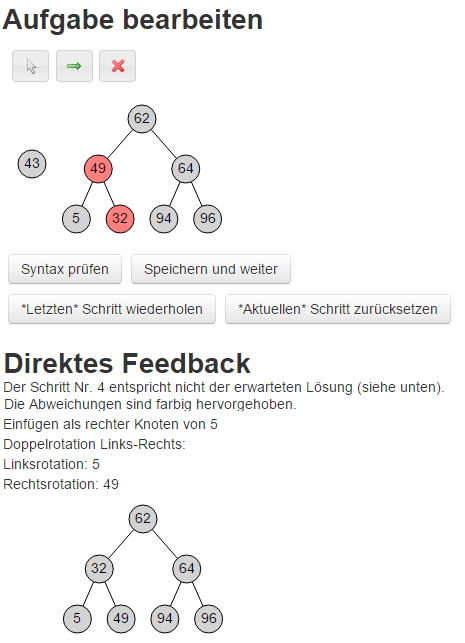
\includegraphics[width=0.5\textwidth]{graphics/editor.jpg}
  \caption{DSBuilder Editor}
  \label{fig:editor}
\end{figure}
Im mittleren Teil der Sicht befindet sich der Editor, in dem der Studierende die Aufgabe bearbeiten kann. Im oberen linken Bereich des Editor befinden sich drei Kn�pfe (vergl. Abb. \ref{fig:editor}), �ber welche der Editiermodus ausgew�hlt werden kann. Der 1. Knopf erm�glicht das verschieben von Konten im Editor, der zweite Knopf erm�glicht das Ziehen von Kanten zwischen zwei Knoten, und der dritte Knopf erm�glicht das Entfernen von Kanten.

Der Drag-and-Drop-Grafikeditor enth�lt zwei bearbeitbare Elemente, die Knoten und die Kanten. �ber Manipulation dieser Elemente sollen Studierende den
Umgang mit Datenstrukturoperationen erlernen. Hierbei k�nnte der Studierende Operationen wie das Einf�gen eines Elements in oder das L�schen eines Elements aus einer Datenstruktur 
praktizieren. In der momentanen Version des EASyDSBuilders kann der Studierende nur das Einf�gen Praktizieren. Weiterhin beginnt in dieser Version jeder Schritt mit dem Ergebnisbaum des zuvor eingereichten Schritts, oder einem Initiierngsbaum,
falls es sich um den  ersten Schritt handelt.
Auf der linken Seite des Editors wird der einzuf�gende Knoten bereitgestellt. Die Aufgabe des Studierenden ist es nun, diesen Knoten an der richtigen 
Stelle in den Baum einzuf�gen. Hierbei kann er sich dem Verschieben der Knoten wie dem L�schen oder neu Ziehen von Kanten bedienen.
Nachdem der Studierende seine Ver�nderungen vorgenommen hat, kann er �ber den Knopf \textit{Syntax pr�fen} den Baum ausbalanciert anzeigen lassen. Auf diese Weise kann der Studierende �berpr�fen, ob die Anwendung den Baum im Sinne des Studierenden verarbeitet hat. Entspricht die �berpr�fte Struktur nicht der Struktur eines Bin�rbaumes, bekommt der Studierende eine Fehlermeldung mit einem Hinweis �ber die Fehlerquelle. Ein Baum wird in diesem Sinne als fehlerhaft angesehen, wenn ein Knoten nicht Teil des Baums ist, oder der Baum zyklisch ist.

Hat der Lehrende bei der Einrichtung des DSBuilders die Option \textit{direktes Feedback} eingestellt, erscheint im Falle einer falschen Eingabe ein Feedbackfeld unterhalb des Editors. In diesem Feedbackfeld wird zu erst ein Informationstext angezeigt, welches das richtige Vorgehen in dem zuvor eingereichtem Schritt beschreibt. Unterhalb dieses Informationstextes ist der korrekte Baum zu sehen. Die falsch eingeordneten Knoten sind rot markiert (vergl. Abb. \ref{fig:editor}). 

\subsection{Einordnung als E-Assessment-Tool}
Datenstrukturen wie Bin�rb�ume sind elementare Bestandteile von Informatikklausuren. Insbesondere der Umgang mit Operationen wie dem Einf�gen oder L�schen von Elementen innerhalb solcher Strukturen erfordert kognitive F�higkeiten. Der EASy-DSBuilder soll hierbei beim Erlernen dieser F�higkeiten innerhalb der Informatikvorlesung unterst�tzen \cite[S. 1]{Usener2014}. In welchen Typ E-Assessment der DSBuilder einzuordnen ist wird im folgenden Abschnitt erl�utert.

In Kapitel \ref{sec:eassessmentEinleitung} wurden bereits die drei Assessmenttypen diagnostisches, formatives und summatives Assessment vorgestellt. Diagnostisches Assessment hat die Aufgabe die F�higkeiten von Teilnehmern vor Beginn einer Lehrveranstaltung zu ermitteln. Die Funktionalit�t des DSBuilders erm�glicht diesen Einsatzzweck, jedoch ist der beabsichtigte der Einsatz w�hrend des Lehr- und Lernbetriebs \cite[S. 1]{Usener2014}. Dies wiederum spricht daf�r, dass der DSBuilder als formatives Assessment eingestuft wird. Das Tool stellt f�r diese Kategorisierung alle geforderten Funktionalit�ten bereit. So kann eingestellt werden, dass der Studierende ein direktes Feedback erh�lt, sodass er sich selbst einsch�tzen kann. Des weiteren kann der Lehrende die Ergebnisse einsehen und somit den Lernstand innerhalb des Kurses einsch�tzen. Wenn die Feedbackfunktion jedoch abgestellt wird, bietet der DSBuilder die Funktionalit�t eines summativen Assessments, da der Lehrende neben der M�glichkeit der Einsichtnahme in die Abgaben auch die M�glichkeit der Bewertung der Abgaben hat.

\subsection{Umsetzung aus technischer Sicht}
\label{sec:technologien}

Das gesamte System um den EASy-DSBuilder besteht backendseitig aus zwei separaten Systemen. Zum einen gibt es das eigentliche Moodlemodul, welches in eine bestehenden Moodelplattform integriert werden kann, zum anderen gibt es einen Datenstruktur-Verarbeitungsservice, welcher als Webservice implementiert ist. Das Moodlemodul hat die M�glichkeit �ber die Moodle-API Daten in einer SQL-Datenbank - beispielsweise einem MySQL-Server - zu hinterlegen. Die Kommunikation zwischen dem Moodlemodul und dem Webservice l�uft �ber das SOAP-Protokoll. Der Webservice ist als WildFly Application Server implementiert und unterliegt somit dem Java-EE7-Standard \cite{wildflyCert}. In Abbildung \ref{fig:technoloieUeberblick} ist dargestellt, wie die unterschiedlichen Technologien in einander greifen.

\begin{figure}[htbp] 
  \centering
     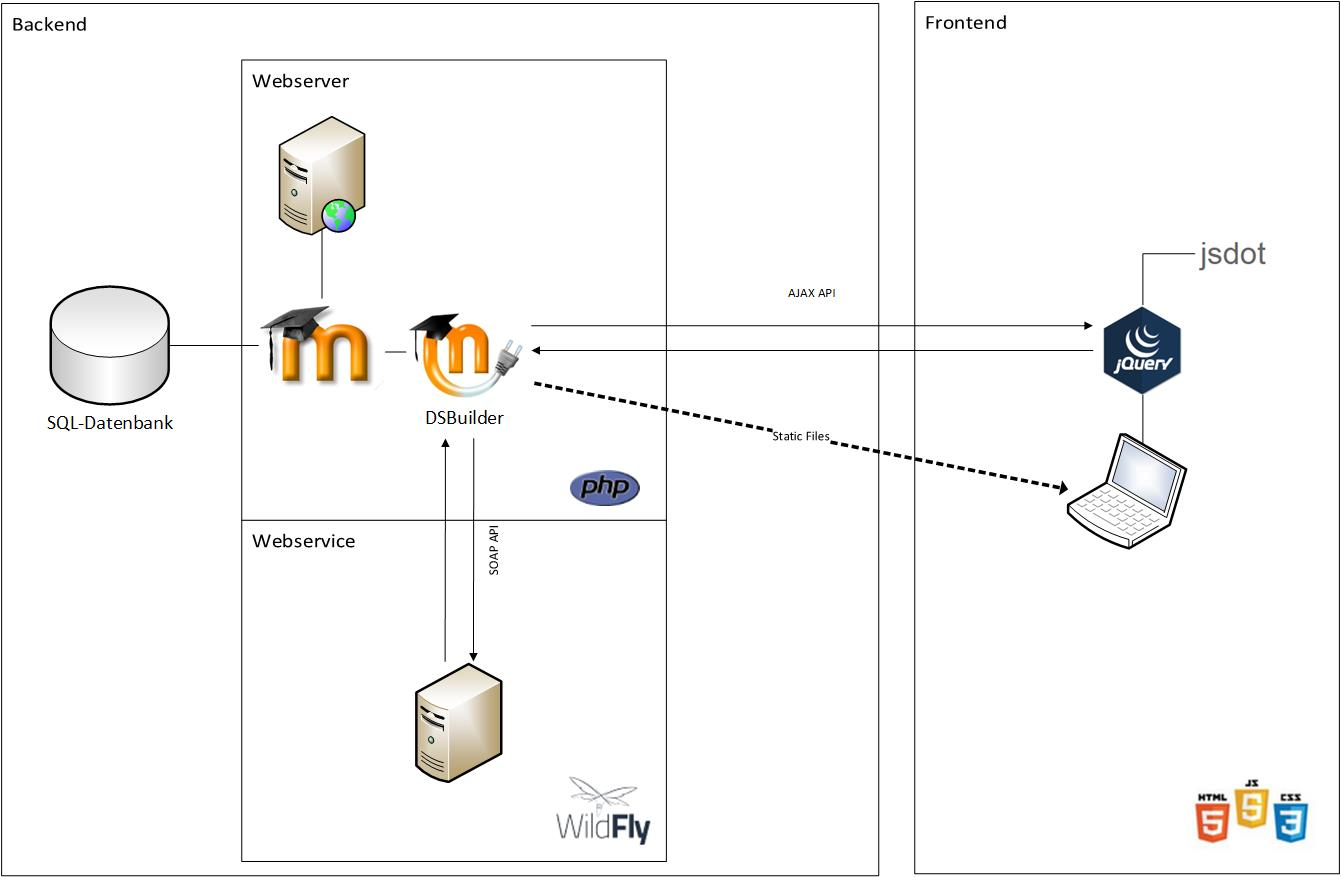
\includegraphics[width=0.9\textwidth]{graphics/UeberblickTechnologien.jpg}
  \caption{Technischer �berblick}
  \label{fig:technoloieUeberblick}
\end{figure}

Auf Clientseite wird HTML mit CSS und JavaScript verwendet, um das Modul f�r den Benutzer darstellen zu k�nnen. Als JavaScript-Frameworks wird jQuery und und als JavaSrcipt-Applikation wird jsdot eingesetzt. �ber jQuery ist die Kommunikation mit dem Moodlemodul �ber das AJAX-Protokoll organisiert. Jsdot dient als Grapheditor.  

\subsubsection{Datenstruktur-Verarbeitungsservice}  
\label{sec:technWebService}


Der Datenstruktur-Verarbeitungsservice hat die Aufgabe Datenstrukturen in Form eines JSON Strings f�r das Moodlemodul bereitzustellen. Hierf�r muss der Lehrende zuvor eine Wrapperdatei auf Basis eines vorgegebenen Interfaces (vergl. Anhang Codebeispiel \ref{code:wrapper}) in Java implementieren und der Anwendung zur Verf�gung stellen. Diese Wrapperklasse dient als Schnittstelle zwischen dem Webservice und der Implementierung der Datenstruktur. Die wichtigen Funktionen, die durch die Implementierung dieses Interfaces zur Verf�gung gestellt werden sollten sind das Hinzuf�gen und L�schen von Schl�sseln, sowie das Erzeugen eines serialisierten JSON Strings aus der Datenstruktur und das Deserialisieren eines JSON Strings in die Datenstruktur.  
 
Um funktionsf�hig zu sein, muss der Datenstruktur-Verarbeitungsservice den vom Lehrenden bereitgestellten Code kompilieren und ausf�hren. Der Verarbeitungsservice ist als separater Webservice implementiert und wird somit von einem anderen Server aus bereitgestellt. Die Separierung des Systems erfolgt aus den Risiken, dass der Code sch�dlich sein oder eine schlechte Ausf�hrungsleistung aufweisen kann. Durch die Trennung der beiden Systeme kann in beiden F�llen Zusammen- oder Performanceeinbr�chen der gesamten E-Learning-Plattform vorgebeugt werden. Weiterhin kann so Datendiebstahl verhindert werden, da in der Verarbeitungsumgebung keine nutzerbezogenen Daten verarbeitet werden. Bei Ausfall des Verarbeitungsservices ist jedoch das Aufrufen eines n�chsten Schrittes nicht mehr m�glich \cite{Usener2014}.

Der Webservice verf�gt �ber die SOAP-Schnittstellen  \textit{analyzeSourceCode}, \textit{assignmentInitialize} und \textit{assignmentIsIntialized}, die zur Initialisierung einer neuen DSBuilder-Instanz be�tigt werden, ebenso wie die SOAP-Schnittstellen \textit{submissionGetNextInput} und \textit{submissionGetInitialDS}, die zur Verarbeitung einer Datenstruktur ben�tigt werden. Um den Webservice nutzen zu k�nnen m�ssen ihm Codedateien zu Verf�gung gestellt werde. �ber den SOAP-Aufruf \textit{analyzeSourceCode} wird die Lesbarkeit der Dateien gepr�ft. Anschlie�end kann �ber den SOAP-Aufruf \textit{assignmentInitialize} der Code compiliert und bereitgestellt werden. Die Ausf�hrung des Codes ist vor jedem Einf�gen, das von einem Studierenden durchgef�hrt wird, notwendig.
So kann �ber den SOAP-Aufruf \textit{submissionGetNextInput} der der n�chste �bungsschritt f�r den Studierenden erhalten werde. Bei der Initialisierung der �bung wird der SOAP-Aufruf \textit{submissionGetInitialDS} ben�tigt. Die Antwort auf diese beiden Aufrufe beinhaltet den neuen Schl�ssel, die serialisierte Datenstruktur und zus�tzliche Hilfe. 


\subsubsection{Moodlemodul backendseitig}
\label{sec:dsbuilderbackend}
Das backendseitige Moodlemodul besitzt die grundlegende Struktur eines Moodlemoduls, wie sie in Kapitel \ref{sec:modularten} dargestellt wurde. Die weiteren, f�r die Funktionalit�t des Moduls wichtigen Dateien sind die Dateien \pfile{renderer.php} und \pfile{render}- \pfile{able.php}, welche den DOM-Code generieren, die Dateien \pfile{ajax\_request.php} und \pfile{ajax\_helper.php}, welche das Handling von AJAX-Anfragen �bernehmen und die Datei \pfile{lib/js\_dot\_convert.php}, welche die Funktionen zur Verarbeitung der Datenstrukturen zur Verf�gung stellt. Im weiteren Verlauf dieses Abschnittes werden diese drei Funktionalit�ten tiefgehender erl�utert und Codeausschnitte exemplarisch vorgestellt.

\paragraph{Generierung des DOM-Codes} \hfill \\
Die Datei, welche f�r die Generierung des DOM-Codes verantwortlich ist, ist die \pfile{renderer.php}. Die Datei \pfile{renderable.php} implemeniert hingegen ein Interface, welches f�r die Verwendung des moodleinternen Renderers notwendig ist \cite{moodleRenderer}. Die in der Datei  \pfile{renderer.php} enthaltende Klasse \pfile{mod\_dsbuilder\_renderer} enth�lt Funktionen zum Erstellen der f�r den DSBuilder ben�tigten Ansichten. So k�nnen �bersichten �ber laufende oder eingereichte Abgaben oder Notentabellen generiert werden.
\begin{figure}[htbp] 
\lstinputlisting[language=PHP, caption=Aufruf zur Initialisierung eines JSDot-Graphs, frame=single, label=code:initGraphEditor]{code/initDSBuilder.php}
\end{figure}
Ebenso k�nnen Ansichten zur Aufgabenbearbeitung generiert werden. Hierbei �bernimmt die Initiierung des Grapheneditors, welche im Quellcode \ref{code:initGraphEditor} dargestellt wird, eine zentrale Rolle. Es wird eine Hilfsfunktion des Moodle-API \cite{moodleJsApi} verwendet, welche die frontendseitige JavaScript-Funktion zur Initialisierung des Grapheneditors anst��t. Die frontendseitige Funktionalit�t wird im Kapitel \ref{sec:dsbuilderfrontend} vertieft.

\paragraph{Modulinterne AJAX-API} \hfill \\
Zur asynchronen Daten�bertragung zwischen Browser und Server stellt das Moodlemodul eine AJAX Api zur Verf�gung. 
\pfile{ajax\_helper.php} definiert.
\begin{figure}[htbp] 
\lstinputlisting[language=PHP, caption=Ausschnitt AJAX API, frame=single, label=code:ajax]{code/ajax.php}
\end{figure}
Der Quellcode \ref{code:ajax} zeigt einen Codeausschnitt aus der \pfile{ajax\_request.php}, in dem die m�glichen Aktionen definiert sind, die nach einer AJAX-Anfrage durchgef�hrt werden k�nnen. Hierbei handelt es sich um die Funktionen, welche �ber die Kn�pfe unterhalb des Grapheneditors (vergl. Kapitel \ref{sec:funktionalitaet}, Abschnitt \textit{Studierender}) angesto�en werden k�nnen. Explizit handelt es sich um die Funktionen \textit{Syntax pr�fen} (Quellcode \ref{code:ajax}, Z. 2), \textit{Speichern und weiter} (Quellcode \ref{code:ajax}, Z. 6) und \textit{Letzten Schritt wiederholen} (Quellcode \ref{code:ajax}, Z. 10). Die jeweils angesto�enen Funktionen sind in der 
Von dort aus werden weitere Funktionen zur Datenstrukturverarbeitung in der Klasse \pfile{jsdot\_graph} angesto�en. Diese Funktionen werden im n�chsten Abschnitt vertiefender behandelt.

\paragraph{Die Datenhaltung} \hfill \\
Das Modul DSBuilders ben�tigt vier Entit�ten f�r seine Datenhaltung. Es handelt sich um die Entit�ten \textit{DSBuilder}, \textit{Assigment File}, \textit{Submission} und \textit{Submission Step}. Die Abbildung \ref{fig:erm} zeigt das Datenmodell des Moduls. 
\begin{figure}[htbp] 
  \centering
     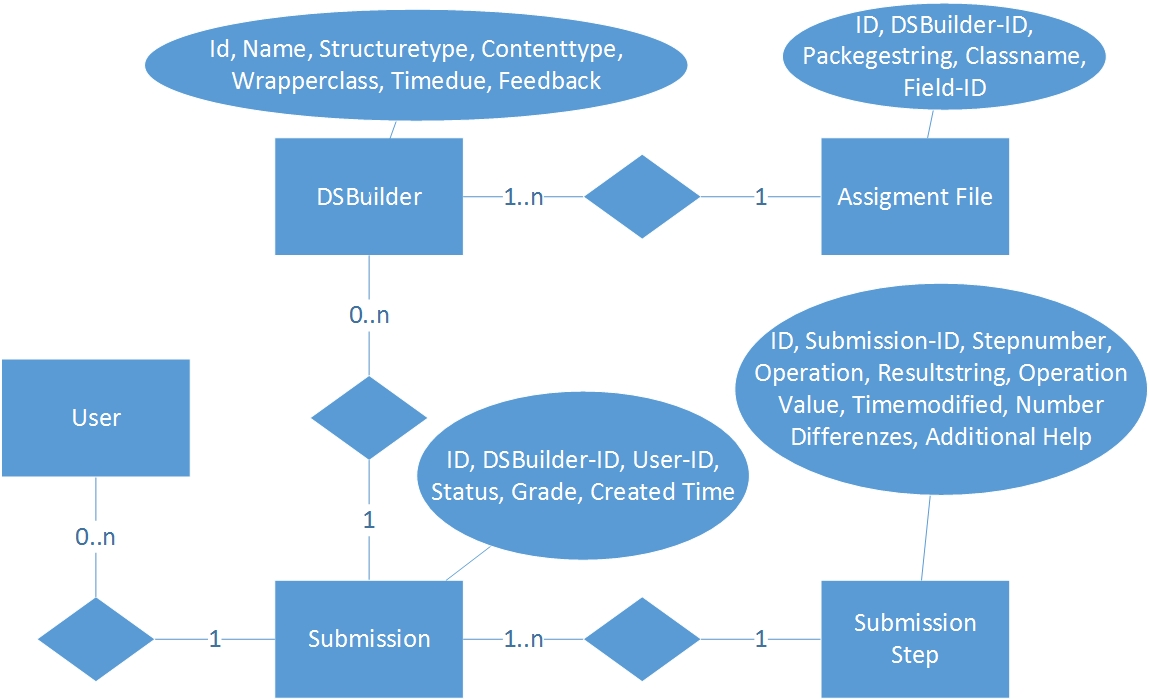
\includegraphics[width=0.9\textwidth]{graphics/ERM.jpg}
  \caption{Datenmodell des DSBuilders}
  \label{fig:erm}
\end{figure}
Nachdem das Modul neu in einem Kurs initialisiert worden ist, wird ein neues Datum der Entit�t \textit{DSBuilder} angelegt. Die der neuen Instanz des Moduls vom Lehrenden zugewiesenen Javadateien werden als Datum der Entit�t \textit{Assigment File}  gespeichert. Sobald Studierende die Instanz nutzen, wird f�r jeden Studierenden mit Vermerk auf die Instanz ein neues Datum der Entit�t \textit{Submission} angelegt. Jeder \textit{Submission} werden \textit{Submission Steps} zugeordnet. Sie beinhalten Informationen �ber die jeweiligen ausgef�hrten Schritte. 

\paragraph{Die Datenstrukturverarbeitung} \hfill \\
In der Datei \pfile{lib/js\_dot\_convert.php} liegt die Funktionalit�t der Datenstrukturverarbeitung. In ihr sind vier Klassen implementiert, von denen die Klasse \pfile{jsdot\_ graph} eine Schnittstelle zur Konvertierung einer Datenstruktur zwischen dem Grapheneditor im Frontend und der Datenhaltung im Backend bietet. Des weiteren repr�sentiert diese Klasse die Datenstruktur, die im jsdot-Editor zur Pr�sentation eines Baumes gebraucht wird. Da ein jsdot-Graph �ber Knoten und Kanten verf�gt, werden diese Elemente in der Datei \pfile{lib/js\_dot\_convert.php} durch die Klassen \pfile{jsdot\_edge} und \pfile{jsdot\_node} repr�sentiert. Spezifischere Erl�uterungen zu den jsdot-Elemente sind in Kapitel \ref{sec:dsbuilderfrontend} zu finden.
Abbildung \ref{fig:umlJsDotConvert} zeigt ein UML-Klassendiagramm der vier Klassen.
\begin{figure}[htbp] 
  \centering
     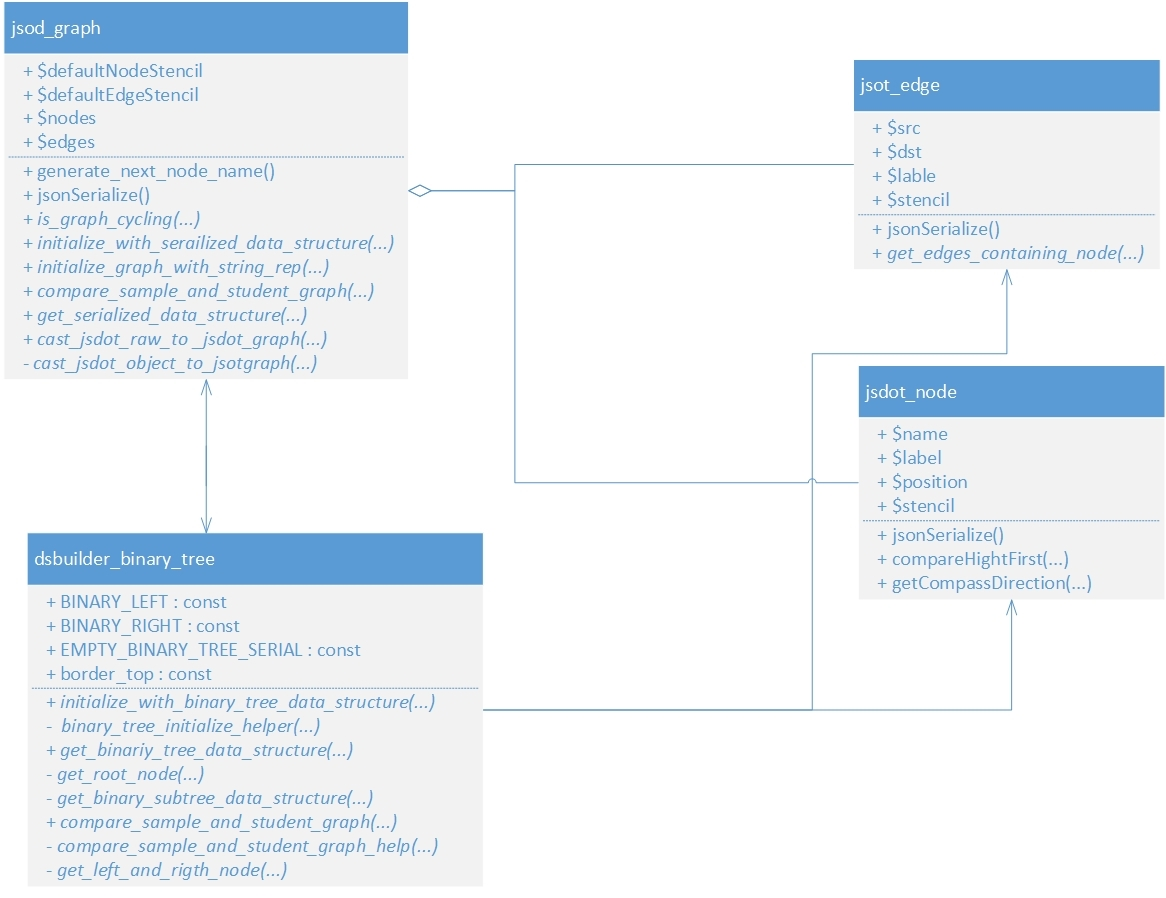
\includegraphics[width=0.9\textwidth]{graphics/UMjsDotConvert1.jpg}
  \caption{UML js\_dot\_convert}
  \label{fig:umlJsDotConvert}
\end{figure}
Die Funktionalit�t zur Umwandlung zwischen Datenstrukturen f�r den jsdot-Editor und den Webservice stellt die Klasse \pfile{dsbuilder\_binary\_tree} bereit. 

Die drei �ffentlichen Funktionen der Klasse \pfile{dsbuilder\_binary\_tree}, die die wichtigen Funktionalit�ten zur Verarbeitung der Datenstruktur bereitstellen, sind die statischen Funktionen 
\textit{initialize\_with\_binary\_tree\_data\_structure(...)}, \textit{get\_bi- nary\_tree\_data\_ structure(...)} und \textit{compare\_sample\_and\_student\_graph(...)}. Hierbei erm�glichen die erste Funktionen die Umwandlung der Datenstruktur, die der Webservice liefert, in die Datenstruktur f�r den jsdot-Editor. Die zweite Funktion erm�glicht die Umwandlung in die umgekehrte Richtung. Die dritte Funktion vergleicht zwei Graphen und markiert die sich unterscheidenden Knoten. Sie wird f�r die Feedbackfunktion genutzt. Im folgenden werden die Funktionen tiefgehender vorgestellt.

\subsubsection{Moodlemodul frontendseitig}
\label{sec:dsbuilderfrontend}
Die im Vordergrund stehende Funktionalit�t des Fronends ist die von der JavaScript-Applikation jsdot bereitgestellte Grapheneditor. In diesem Grapheneditor  werden von Elemente zur Verf�gung gestellt, die vom Studierenden bearbeitet werden k�nnen. 
Die Funktionalit�t zur Verarbeitung der Nutzereingaben wird �ber die Datei \pfile{dsbuilder.js} bereitgestellt.
Des weiteren stellt diese Datei die AJAX-Kommunikation zur Verf�gung.

\paragraph{Der Grapheneditor} \hfill \\
Der Grapheneditor wird durch die JavaScript-Applikation jsdot bereitgestellt. So kann jsdot �ber das HTML-Element \textit{svg} Knoten und Kanten bereitstellen, die editierbar sind. Aus diesen Elementen k�nnen Strukturen wie Graphen, B�ume oder Listen erstellt werden. Der Codeauszug \ref{code:initJsDot} zeigt die Initialisierung eines neuen jsdot-Graphen. 
\begin{figure}[htbp] 
\lstinputlisting[language=JavaScript, caption=Initiierung eines JsDot-Graphs, frame=single, label=code:initJsDot]{code/initJsDot.js}
\end{figure}
Weiterhin stellt jsdot eine API zur Verf�gung. �ber diese API k�nnen  neue Elemente zu einem Graphen hinzugef�gt werden. Ebenso k�nnen bestehende Elemente ge�ndert oder ausgelesen werden. Au�erdem kann bei der Initialisierung eines Graphen eingestellt werden, ob der Graph im Bearbeitungsmodus oder im Anzeigemodus bereitgestellt wird. Codebeispiel \ref{code:initJsDot} zeigt die Initialisierung eines Graphen im Bearbeitungsmodus. 
So wird der Editiermodus verwendet, um einen editierbaren Graphen f�r die Aufgabenbearbeitung zur Verf�gung zu stellen (vergl. Kapitel \ref{sec:funktionalitaet} Abb. \ref{fig:editor} oben). Der Anzeigemodus wird hingegen f�r das Feedback verwendet (vergl. Kapitel \ref{sec:funktionalitaet} Abb. \ref{fig:editor} unten). Im Frontend findet keine Verarbeitung der Graphen-Datenstruktur statt. Die Graphen-Datenstruktur wird �ber die im folgenden Abschnitt erl�uterte AJAX-API an das Backend gesendet und dort verarbeitet (vergl. Kapitel \ref{sec:dsbuilderbackend} Abschnitt \textit{Datenstrukturverarbeitung}).

\paragraph{AJAX-Api des Frontends} \hfill \\
Das Frontend stellt eine AJAX-API zur Echtzeitkommunikation mit dem Moodlemodul bereit. �ber die Kn�pfe unterhalb des Grapheneditors (vergl. Kapitel \ref{sec:funktionalitaet}, Abschnitt \textit{Studierender}) k�nnen die Funktionen der API angesto�en werden. Die Verarbeitung der AJAX-Anfragen wurde bereits in Kapitel \ref{sec:dsbuilderbackend} im Abschnitt \textit{Modulinterne AJAX-API} erl�utert. �ber AJAX-Anfragen werden Informationen wie die Graphen-Datenstruktur, das Feedback und m�gliche Fehler �bertragen.
\section{Konzeptionelle Anforderungen an ein E-Learning-Modul zum Assessment von
B-Baum-Datenstrukturen}
\label{sec:anforderungen}

In diesem Kapitel werden die bestehenden Anforderungen an ein E-Learning-Modul zum Assessment von B-Baum-Datenstrukturen vorgestellt und n�her erl�utert. Da es sich bei diesem E-Learning-Modul um den bereits existierenden EASy-DSBuilder handelt, welcher lediglich um die Funktion des Assessments von
B-Baum-Datenstrukturen erweitert werden muss, stellt das Kapitel \ref{sec:neuanforderungen} die Neuanforderungen an den EASy-DSBuilder vor. Anschlie�end wird in Kapitel \ref{sec:konzeptGrapheneditor} tiefgehender auf die Anforderungen des Grapheneditors eingegangen.


\subsection{Neuanforderungen an den EASy-DSBuilder}
\label{sec:neuanforderungen}
In diesem Kapitel werden die Anforderungen an die Erweiterungen des EASy-DSBuilders vorgestellt und n�her erl�utert. Die Hauptanforderung lautet:
\begin{quote}
Der EASy DSBuilder soll um die Datenstruktur B-Baum erweitert werden.
\end{quote}
Aus dieser Hauptanforderung lassen sich weitere Unteranforderungen Ableiten.
\paragraph{(1) Dem Studierenden muss ein Assessment einer B-Baum-Datenstruktur durchf�hren k�nnen} 
\begin{quote}
Dem Studierenden wird eine graphische Oberfl�che bereitgestellt, auf der ein Assessment einer B-Baum-Datenstruktur m�glich ist. Hierf�r braucht es insbesondere einen Editor, der eine B-Baum-Grundstruktur mit Kanten und Knoten bestehen. Auf dieser soll es m�glich sein Schl�ssel zu positionieren. 
\end{quote}
Mit dieser Anforderung ist die grundlegende Funktionalit�t des Moduls, die das Assessment von B-Baum-Datenstrukturen erm�glichen soll, begr�ndet. Wie in Kapitel \ref{sec:funktionalitaet} erl�utert verf�gt der EASy-DSBuilder �ber die Funktionalit�t des Assessments von AVL-B�umen. So soll das Assessment von B-Baum-Datenstrukturen den selben Funktionalen Umfang des AVL-Baum-Assessments haben. Hierzu geh�ren folgende Funktionen. Das Assessment geht �ber 10 Schritte, in denen der Baumstruktur jeweils ein neuer Sch�ssel hinzugef�gt werden soll. Der Studierende erh�lt einen �berblick �ber den aktuellen Stand der Aufgabe, die er bearbeitet. Der Studierende erh�lt einen Editor zum Assessment  von B-Baumstrukturen. Der Studierende kann die Syntax seiner Eingabe pr�fen. Der Studierende kann seine Eingabe abgeben. Der Studierende kann den aktuellen Schritt seiner Eingabe zur�cksetzen. Der Studierende kann den vorherigen Schritt seiner Eingabe zur�cksetzen. Es soll die M�glichkeit des Feedbacks gegeben werden. Im folgenden Verlauf wird detaillierter auf die soeben genannten Anforderungen eingegangen.

\paragraph{() Das Assessment soll zehnschrittig sein}
\begin{quote}
Das Assessment soll �ber 10 Schritte gehen, in denen der Baumstruktur pro Schritt jeweils ein neuer Sch�ssel hinzugef�gt wird.
\end{quote}
Ebenso wie beim Assessment des AVL-Baums soll das Assessment des B-Baums �ber zehn Schritte gehen. Pro Schritt wird dem Studenten hierbei ein neuer Schl�ssel zur Verf�gung gestellt, die er in den bereits vorhanden B-Baum einf�gen k�nnen soll. Nachdem die zehn Schritte absolviert sind, soll der Studierende dar�ber informiert werden, dass er die gesamte Aufgabe absolviert hat.


\paragraph{() Studierende soll �berblick �ber aktuellen Aufgabenstand erhalten}
\begin{quote}
Der Studierende soll die M�glichkeit erhalten einen �berblick �ber den aktuellen Stand der Aufgabe, die er bearbeitet, zu bekommen.
\end{quote}
Ebenso wie beim Assessment des AVL-Baums soll das Assessment des B-Baums �ber eine �bersicht �ber dein aktuellen Stand der Aufgabe bereitstellen. Auf dieser �bersicht erh�lt der Studierende Informationen dar�ber, wie viel Prozent er bereits absolviert hat, in welchem Schritt er sich befindet und welcher Schl�ssel in diesem Schritt zum Einf�gen bereitgestellt wurde.


\paragraph{() Der Studierende soll einen Editor zum Assessment  von B-Baumstrukturen erhalten}
\begin{quote}
Der Studierende soll die M�glichkeit bekommen, eine B-Baum-Datenstruktur innerhalb eines Editors so zu bearbeiten, dass er die Aufgabenstellung jedes Schrittes l�sen kann.
\end{quote}
Ebenso wie beim Assessment des AVL-Baums soll das Assessment des B-Baums �ber einen Editor verf�gen, in dem man eine B-Baum-Datenstruktur bearbeiten kann. 
Die Elemente, die durch den Editor bereitgestellt werden sollen, sind Kanten, Knoten und Schl�ssel. Es soll m�glich sein, aus diesen Elementen eine syntaktisch korrekten B-Baum zu erstellen. Des weiteren muss der Editor Funktionalit�ten bereitstellen, die das Einf�gen eines neuen Schl�ssels in einen bereits bestehenden B-Baum erm�glichen.


\paragraph{() Der Studierende soll die Syntax seiner Eingabe pr�fen k�nnen}
\begin{quote}

\end{quote}

\paragraph{() Der Studierende soll seine Eingabe abgeben k�nnen}
\begin{quote}

\end{quote}



\paragraph{() Der Studierende soll den aktuellen Schritt seiner Eingabe zur�cksetzen k�nnen}
\begin{quote}

\end{quote}

\paragraph{() Der Studierende soll den vorherigen Schritt seiner Eingabe zur�cksetzen k�nnen}
\begin{quote}

\end{quote}

\paragraph{() Es soll die M�glichkeit des Feedbacks gegeben werden}
\begin{quote}

\end{quote}

\paragraph{() }
\begin{quote}

\end{quote}

\paragraph{() }
\begin{quote}

\end{quote}

\paragraph{(2) Der Lehrende soll eine Auswahlm�glichkeit erhalten, zwischen Datenstrukturen w�hlen zu k�nnen}
\begin{quote}
Der Lehrende soll bei Einrichtung einer neuen Instanz des DSBuilders aus einer Liste mit allen verf�gbaren Datenstrukturen die Auswahl treffen k�nnen, mit welcher Datenstruktur die Anwendung dem Studierenden bereitgestellt wird.
\end{quote}



\begin{itemize}
\item editirbare graphische Oberfl�che zur Erstellung von B-B�umen
\item Funktionalit�t soll beibehalten werden:
\begin{itemize}
\item Kommunikation Moodle <---> Web-Server
\item Schritte werden gespeichert
\item Eingabe �berpr�fen
\item Feedback
\item farbige Markierung falscher Knoten
\item Schritt zur�ck
\end{itemize}
\item Lehrender: Auswahl zwischen Typ
\item alles in einer akzeptablen Zeit.
\end{itemize}

\subsection{Spezifizierung der konzeptionellen Anforderungen des Grapheneditors}
\label{sec:konzeptGrapheneditor}
Wenn man die Anforderungen aus Kapitel \ref{sec:neuanforderungen} auf eine Kernanforderung reduziert, so kann sie darin verstanden werden, dass dem Studierenden ein graphischer Editor zur Verf�gung gestellt werden soll, �ber den ein B-Baum erweitert werden kann. Vergleicht man eine B-Baum mit dem bereits implementierten AVL-Baum, so verf�gt der B-Baum �ber eine weitere editierbare Komponente. Beim AVL-Baum sind Knoten und Sch�ssel durch ein \textbf{eins-zu-eins-Mapping} unver�nderbar miteinander verbunden, beim B-Baum kann ein Knoten jedoch mehrere Schl�ssel enthalten, welche aber auch nicht fest an diesen Knoten gebunden sind. Die daraus resultierende Herausforderung ist die drei Komponenten Kante, Knoten und Schl�ssel dem Studierenden so zur Verf�gung zu stellen, dass der Studierende die Komponenten m�glichst intuitiv nutzen kann. Die JavaScript-Applikation jsdot soll dabei beibehalten werden. Es ergaben sich die M�glichkeiten, einen B-Baum komplett aus editierbaren jsdot-Elementen zu implementieren, oder eine B-Baumstruktur in den Hintergrund des Editors zu legen, auf dem die Schl�ssel richtig eingeordnet werden m�ssen. Im Folgenden werden Vor- und Nachteile beider M�glichkeiten vorgestellt.

\paragraph{B-Baum aus jsdot-Elementen} \hfill \\
Jsdot bietet die M�glichkeit neben runden auch rechteckige Knoten zu erstellen. Aus diesen k�nnten Knoten generiert werden. Auf diese Weise k�nnten Studierende eine B-Baumstruktur auf der Basis dieser Knoten und Kanten erstellen, um darauf die jeweiligen Schl�sselelemente richtig zu positionieren. 

Jedoch ergeben sich daraus mehrere Probleme. Zum einen ist die Umsetzung der Positionierung der abw�rtsgerichteten Kanten ein Problem. Idealtypisch ist die Positionierung der abw�rtsgerichteten Kanten am Anfang oder am Ende eines Knotens oder zwischen zwei Schl�sseln (vergl. Abb. \ref{fig:bbaum}). 
Dies ist jedoch ohne einen gr��eren Eingriff in die jsdot-Implementierung nicht m�glich. Alternativ k�nnen die abw�rtsgerichteten Kanten an die Schl�ssel geh�ngt werden, wobei der erste oder letzte Schl�ssel eines Knotens �ber zwei abw�rtsgerichtete Kanten verf�gt. Die Kanten k�nnen dann wie zuvor an Knoten enden. Jedoch kann nicht unterbunden werden, dass Schl�ssel oder Kanten untereinander im nicht beabsichtigten Sinn verbunden werden. Daraus resultiert, dass eine Gro�zahl an m�glichen falschen Eingabem�glichkeiten �berpr�ft werden m�sste. Auch k�nnte diese Vorgabe die Usability beeintr�chtigen, da sich die geforderte Benutzung der einzelnen Elemente seitens des Studierenden nicht eindeutig nachvollziehbar herausstellen k�nnte. Des Weiteren bereitet die H�henhierarchie der einzelnen jsdot-Elemente Probleme. So ist es auf Grund fehlender Dokumentation bez�glich der H�henhierarchie einzelner Elemente schwer umsetzbar Schl�ssel so zu definieren, dass sie Knoten durchgehend �berlappen.



\paragraph{B-Baumstruktur im Hintergrund} \hfill \\
Die Baumstruktur im Hintergrund bietet den Vorteil, dass nur noch die einzelnen Schl�ssel editierbar sein m�ssen, der Studierende folglich nur noch die Schl�ssel an die richtige Position bringen muss. Dies bietet den Vorteil, dass die Richtigkeit �ber die absolute Position, und nicht Position relativ zu anderen Schl�sseln, gepr�ft werden kann.  Es ergeben sich  zwei M�glichkeiten eines Hintergrundgraphen. Es kann entweder ein statischer Baum, der durchgehend die gesamte Struktur aufweist, oder ein dynamischer Baum, der sich der Eingabe des Studierenden anpasst,  implementiert werden. Ein statischer Baum erfordert weniger Implementierungsarbeit, ein dynamischer Baum erh�ht jedoch die �bersichtlichkeit, da nur ben�tigte Teile des Baums angezeigt werden. Au�erdem bietet ein dynamischer Baum dem Studierenden die Chance die Entwicklung eines B-Baums besser zu veranschaulichen.  implementiert \textbf{kann man das so Schreiben --> ist ja nur meine Meinung} Diesen Vorteilen steht jedoch gegen�ber, dass der Studierende aus didaktischer Sicht in seinen Bearbeitungsm�glichkeiten eingeschr�nkt wurde. Eingeschr�nkt aus didaktischer Sicht bedeutet in diesem Kontext, dass den Studierenden w�hrend in der soeben beschriebenen Aufgabenbearbeitung im Verglich zur papierbasierten Aufgabenbearbeitung Bearbeitungsvariationen bei der L�sungsfindung vorenthalten werden. Insbesondere kann der Studierende die Baumstruktur nicht mehr falsch aufbauen, sodass die Hintergrundstruktur des B-Baums zur Reduktion m�glicher Fehlerquellen f�hrt.

\paragraph{Ergebnis} \hfill \\
Insbesondere der B-Baum aus jsdot-Elementen bringt verschiedene Herausforderungen mit sich. So ist es in dieser Variante auf Grund der Vielzahl von Elementen schwierig eine einfach zu verstehende und zu benutzende graphische Oberfl�che zu bieten. Dem gegen�ber steht die einfach zu bedienende graphische Oberfl�che mit einer B-Baumstruktur im Hintergrund, die dem Studierenden jedoch striktere Vorgaben in der Benutzung vorgibt und somit Fehlerquellen reduziert. Die hier vorliegende Situation beschreibt einen Trade-off zwischen geringer Usability mit einem hohen Ma� an Bearbeitungsvariationen und einer hohen Usabiltiy mit einem geringeren Ma� an Bearbeitungsvariationen. Wie die Auswertung der Fallstudie �ber die Nutzung des EASy-DSBuilders zeigte sorgte besonders die gute Usability f�r hohe Akzeptanz bei den Studierenden\cite[S. 5]{Usener2014}. Auch in der neuen Anwendung soll der Akzeptanz eine hohe Priorit�t zugeschrieben werden, sodass trotz der Vereinfachung der Aufgabe durch die Reduktion m�glicher Fehlerquelle der Editor mit Hintergrundstruktur dem Editor, in dem alle Elemente bewegbar sind, vorzuziehen ist. 
\section{Umsetzung der �nderungsanforderungen}
Dieses Kapitel stellt die Stellen vor, an denen �nderungen vorgenommen werden mussten und erl�utert die Ursachen, auf Grund derer die �nderungen vorgenommen werden mussten. Hierzu wird zu erst in Abschnitt \ref{sec:umsetzungUeberblick} ein �berblick �ber die notwendigen �nderungen und Erweiterungen gegeben. In den restlichen Abschnitten wird tiefgehender auf die wichtigen �nderungen und Erweiterungen eingegangen. Dabei wird zuerst die Funktionalit�t erl�utert. Zur Verdeutlichung werden anschlie�end exemplarisch Ausschnitte aus der Implementierung vorgestellt.




\subsection{�berblick �ber �nderungen}
\label{sec:umsetzungUeberblick}
In diesem Abschnitt wird ein grundlegender �berblick �ber alle �nderungen gegeben, die in dem Moodlemodul EASy-DSBuilder vorgenommen wurden, um die Funktionalit�t des Assessments von B-Baum-Datenstrukturen.

F�r die Verwendung des EASy-DSbuilders ist eine Initialisierung seitens eines Lehrenden n�tig. In der alten Version konnten die in Kapitel \ref{sec:funktionalitaet} beschriebenen Eigenschaften �bergeben werden. Es konnte jedoch noch nicht zwischen Datenstrukturen gew�hlt werden. So wurde in der alten Version als Datenstrukturtyp defaultm��ig \textit{Tree} �bergeben. An dieser Stelle musste eine Auswahlm�glichkeit f�r Datenstrukturen in der Erstellungsmaske des Moduls implementiert werden. Die Auswahlm�glichkeit wurde als Dropdown-Men� umgesetzt, wobei die in der Datei \pfile{dsbaStructureType.php} definierten Konstanten als Datenstrukturtypen zur Auswahl gestellt werden.

Nachdem eine Instanz des EASy-DSBuilders erzeugt wurde, muss dem Modul jedoch zur Durchf�hrung eines Assessments eine Datenstruktur seitens des Daten- strukturverarbeitungs-Webservices bereitgestellt werden. Die zur Kommunikation zwischen Moodlemodul und Webservice verwendete Datenstruktur wird in Abschnitt \ref{sec:datenstruktur} vorgestellt. An der Funktionalit�t des Datenstrukturverarbeitungs-Webservice sollte nichts ge�ndert werden. Fehler, die w�hrend der Entwicklung auftraten, wurden behoben. Zur Endwicklung des Moodlemoduls musste jedoch die Datenstruktur eines B-Baums in Java implementiert werden, damit die Funktionen des Webservices bereitgestellt werden konnten. \textbf{�ber die B-Baum Implementierung schreiben?}

Die wichtigen Erweiterungen zur Bereitstellung der Funktionalit�t eines Assessments von B-Baum-Datenstrukturen wurde im Moodlemodul fronend- und backendseitig implementiert. Hierbei steht frontendseitig die Erweiterung des Grapheneditors im Vordergrund, welche ausf�hrlich im Abschnitt \ref{sec:erweiterungEditor} erl�utert wird. Des Weiteren war die Implementierung einer Verarbeitung der Datenstruktur n�tig, sodass zwischen der vom Webservice stammenden Datenstruktur und der f�r den Editor gebrachten Datenstruktur gewandelt werden konnte. Diese Funktionalit�t wird ausf�hrlicher in Abschnitt \ref{sec:strukturverarbeitung} erl�utert. 
Des weiteren wurden noch folgende kleinere Ver�nderungen vorgenommen. In der Datei \pfile{renderer.php}, in der die Ansicht generiert wird, wurde eine Fallentscheidung f�r die Anzeige des Grapheneditors implementiert. Dies ist damit begr�ndet, dass der B-Baum-Editor, wie in Kapitel \ref{sec:konzeptGrapheneditor} begr�ndet, zwei �bereinander liegende jsdot-Editoren ben�tigt. Die �berlagerung der zwei Editoren wurde mit \textit{CSS} umgesetzt.
Weiterhin wurde die AJAX-Api angepasst. Die minimale �nderung bestand darin, dass eine weitere Information �bergeben wird, auf die der B-Baum-Editor aufbaut. N�heres dazu ist in Abschnitt \ref{sec:editorImplemenierungsdetails} zu finden. 

\subsection{Datenstruktur f�r die \\Moodlemodul-Webserice-Kommunikation}
\label{sec:datenstruktur}
Die Datenstruktur, die in in der Kommunikation zwischen Moodlemodul und Webservice eingesetzt wird, spielt eine fundamentale Rolle in der Gesamtanwendung EASy-DSBuilder. Diese Datenstruktur muss in einem JSON-kompatiblen Format alle notwendigen Informationen �ber die zu verarbeitende Baumstruktur beinhalten. Im Falle des B-Baums muss die Datenstruktur als zentrales Element den Knoten mit der jeweiligen Anzahl an Schl�sseln wiedergeben. Des weiteren muss die Datenstruktur noch die Kindsknoten der Wurzelknotens beinhalten, die wiederum richtig positioniert werden m�ssen. So k�nnen die Kindsnoten als linkes oder rechtes Kind des Wurzelknotens positioniert werden. Weiterhin gibt es noch Kindsknoten, die zwischen den einzelnen Schl�sseln des Wurzelknotens positioniert werden (vergl. Kapitel \ref{sec:bbaum}). 

Auf Basis dieser Grundlage wurde zur Abbildung eines B-Baums ein Array als Datenstruktur ausgew�hlt. Dieser Array ist bei einem B-Baum \textit{T} mit einer H�he gr��er eins wie folgt aufgebaut. Erstes Element des Arrays, welches die oberste Wurzel des B-Baums \textit{T} repr�sentiert, ist der linke Kindsknoten der Wurzel. Anschlie�end folgt der erste Schl�ssel der Wurzel, dem ein weiterer Kindsknoten nachfolgt. Diese Abfolge aus Sch�ssel und Kindsknoten erfolgt so lange, bis das Array mit dem rechten Kindsknoten der Wurzel abschlie�t. Die jeweiligen Kindsknoten sind nach der selben Struktur des Wurzelknotens aufgebaut. Eine m�gliche Repr�sentation eines B-Baums durch diese Datenstruktur kann wie folgt aussehen:
\begin{quote}
$[[["16","19"],"31",["37","41"]],"50",[["56"],"86",["96"]]]$
\end{quote} 

Die so eben gezeigte Datenstruktur zeigt einen B-Baum der H�he drei. Der oberste Wurzelknoten enth�lt den Sch�ssel $"3"$. Die Wurzel hat das linke Kind $[["16","19"],"31",["37","41"]]$ und das rechte Kind $[["56"],"86",["96"]]$, welche jeweils separat betrachte einzelne B-B�ume darstellen. Diese Beispiel verdeutlicht anschaulich den rekursiven Aufbau dieser Datenstruktur. Abgeschlossenen wird die Struktur durch kinderlose Knoten, wie sie im vorgestellten B-Baum beispielsweise durch den Knoten $["16","19"]$ repr�sentiert werden. Diese Datenstruktur steht wiederum in einem weiteren Array mit der L�nge zwei an erster Position. An zweiter Position wird die Ordnungszahl \textit{k} (vergl. Kapitel \ref{sec:bbaum}) abgelegt.


\subsection{Datenstrukturverarbeitung backendseitig}
\label{sec:strukturverarbeitung}

Die in diesem Abschnitt vorgestellten �nderungen beziehen sich auf die in Kapitel \ref{sec:dsbuilderbackend} unter Abschnitt \textit{Datenverarbeitung} vorgestellte Funktionalit�t. Bei der Datei, in der �nderungen vorgenommen wurden handelt es sich um die \pfile{lib/js\_dot\_ convert.php}. In ihr befinden sich in der alten Version des EASy-DSBuilders die Klassen \pfile{jsdot\_graph}, \pfile{jsdot\_edge}, \pfile{jsdot\_node} und \pfile{dsbuilder\_binary\_tree}. Die Klasse \pfile{jsdot\_graph} dient als Schnittstelle zum restlichen Modul und verwaltet den jsdot-Graph. Zum Umgang mit �bergebenen Datenstrukturen bedient die Klasse sich im Fall von Bin�rb�umen der Klasse \pfile{dsbuilder\_binary\_tree}. Die nun vorgenommene Erweiterung enth�lt die Implementierung der Klasse \pfile{dsbuilder\_b\_tree}. Diese neu implementierte Klasse orientiert sich stark an der Klasse \pfile{dsbuilder\_ binary\_tree}. Sie stellt die selben Funktionen bereit,  nur dass die Funktionen in der Klasse \pfile{dsbuilder\_b\_tree} dem Umgang mit B-Baum-Datenstrukturen dienen.

Die drei �ffentlichen Funktionen der Klasse \pfile{dsbuilder\_b\_tree} sind die statischen Funktionen 
\textit{initialize\_with\_b\_tree\_data\_structure(...)}, \textit{get\_b\_tree\_data\_ structure(...)} und \textit{compare\_sample\_and\_student\_graph(...)}. Hierbei erm�glichen die ersten beiden Funktionen die Umwandlung der Datenstruktur, sodass mit der Datenstruktur in den beiden Anwendungsf�llen Grapheneditor und Webservices gearbeitet werden kann. Die dritte Funktion vergleicht zwei Graphen und markiert die sich unterscheidenden Knoten. Sie wird f�r die Feedbackfunktion genutzt. Im folgenden werden die Funktionen tiefgehender vorgestellt.

Die Funktion \textit{initialize\_with\_b\_tree\_data\_structure(...)} initialisiert einen neuen \pfile{jsdot\_graph} anhand der in Kapitel \ref{sec:datenstruktur} vorgestellten serialisierten Datenstruktur. Der Funktion k�nnen drei Paramieter �bergeben werden. Die �bergabe einer serialisierte Datenstruktur ist verpflichtend. Ansonsten kann �bergeben werden, wie viel Abstand der Baum im Editor auf der x-Achse zum linken Rand und auf der y-Achse zum oberen Rand haben soll. Standardm��ig werden 50 Pixel f�r die x-Achse und 25 Pixel f�r die y-Achse �bergeben. Jedoch handelt es sich bei der Funktion \textit{initialize\_with\_b\_tree\_data\_structure(...)} nur um eine Wrapperfunktion. Die eigentliche Umwandlung einer serialisierten Datenstruktur in einen \pfile{jsdot\_graph} geschieht in der Hilfsfunktion \textit{b\_tree\_initialize\_helper(...)}. Quellcode \ref{code:bTreeInitHelper} zeigt einen Ausschnitt der Hilfsfunktion.
\begin{figure}[htbp] 
\lstinputlisting[language=PHP, caption=Ausschnitt \textit{b\_tree\_initialize\_helper(...)}, frame=single, label=code:bTreeInitHelper]{code/bTreeInitHelper.php}
\end{figure}
Da es sich bei der serialisierten Datenstruktur um eine rekursiv aufgebaute Datenstruktur handelt ist die Verarbeitung dieser Struktur ebenfalls rekursiv aufgebaut. Der Hilfsfunktion wird eine serialisierte B-Baum-Datenstruktur �bergeben. Wie in Kapitel \ref{sec:datenstruktur} beschrieben besteht die Datenstruktur einem Array, welches Schl�ssel und Kindsknoten-Arrays des Wurzelknotens enth�lt. Auf Grund dieser Struktur wird jedes Element des Wurzelknoten-Arrays durchlaufen (Z. 4). Hierbei werden die einzelnen Knoten-Arrays des �bergebenen B-Baums durch die Variable \pfile{\$json\_row} widergespiegelt. F�r jedes Element in dem jeweiligen Array erfolgt eine Fallunterscheidung, in der gepr�ft wird, ob es sich bei dem jeweiligen Element um ein \textit{String} handelt. Ist das jeweilige Element ein \textit{String} (Z. 5), so muss es sich um einen Schl�ssel im Array handeln. In diesem Fall wird ein neues \pfile{jsdot\_node} initialisiert und den Knoten des \pfile{\$jsdot\_graph} �bergeben (Z. 6 f.). Es werden hierbei jeweils Name, Schl�ssel und Position an den Knoten �bergeben. Wie die Position bestimmt wird, wird in Kapitel \ref{sec:positionierung} erl�utert. Handelt es sich nicht um einen \textit{String}, so muss es sich um ein Kindsknoten-Array handeln. In diesem Fall ruft die Hilfsfunktion sich selber auf, damit die Kindsknoten-Arrays auf die selbe Weise verarbeitet werden k�nnen. Quellcode \ref{code:rekursiverAufrufInitHelper} zeigt den rekursiven Aufruf in seiner Gesamtheit. 
\begin{figure}[htbp] 
\lstinputlisting[language=PHP, caption=rekursiver Aufruf aus Quellcode \ref{code:bTreeInitHelper} in Z. 10, frame=single, label=code:rekursiverAufrufInitHelper]{code/rekursiverAufrufInitHelper.php}
\end{figure}
Der erste �bergebene Parameter ist wieder der in Funktion \textit{initialize\_with\_b\_tree\_data\_structure(...)} initialisierte \pfile{jsdot\_graph}. Der zweite Parameter ist das Kindsknoten-Array. Die n�chsten beiden Parameter beschreiben die Position des Arrays. Als erstes wird die H�he �bergeben, die eine gr��er als die momentane H�he ist. Danach wird die Position innerhalb einer Schicht weitergegeben. \pfile{\$index\_node} sagt dabei aus, um den wievielten Kindsknoten es sich handelt. \pfile{\$indes\_array} zeigt die Position des Wurzelknotens innerhalb der Schicht auf. Diese muss noch mit der Ordnungszahl \pfile{\$t} multipliziert werden, damit die richtige Position f�r den Kindsknoten gefunden wird. Die Summe bildet schlie�lich die Finale Position. Die restlichen Parameter werden unver�ndert weitergegeben.
Zum Abbruch der Funktion dienen die kinderlosen Knoten, da in ihnen keine Kindsknoten-Arrays zum weiteren rekursiven Aufruf vorhanden sind.

Die Funktion \textit{get\_b\_tree\_data\_ structure(...)} wandelt wiederum eine \pfile{jsdot\_graph}-Datenstruktur in eine serialisierte Datenstruktur f�r den Webservice um. Quellcode \ref{code:getBTreeDataStructure} zeigt die gesamte Funktion. 
\begin{figure}[htbp] 
\lstinputlisting[language=PHP, caption=\textit{get\_b\_tree\_data\_ structure(...)}, frame=single, label=code:getBTreeDataStructure]{code/getBTreeDataStructure.php}
\end{figure}
So wird der \pfile{jsdot\_graph} als erstes in die Form \glqq Knoten pro Schicht\grqq umgewandelt (Z. 2). Da diese Form bereits aus Kapitel \ref{sec:editorImplemenierungsdetails} bekannt ist, und die Umwandlung hier �quivalent verl�uft, wird an dieser Stelle nicht weiter darauf eingegangen. Wichtig f�r diese Funktion ist jedoch noch, dass in ihr die Richtigkeit der Syntax des B-Baums gepr�ft wird. Es wird gepr�ft, ob alle Schl�ssel Teil des Baums sind, ob alle Knoten die maximale Anzahl an Schl�sseln nicht �berschreiten und ob der Baum ausbalanciert ist. Anschlie�end wird die rekursive Hilfsfunktion \textit{b\_tree\_structure\_helper(...)} aufgerufen, die die eigentliche Umwandlung umsetzt. Die Hilfsfunktion wird mit dem Wurzelknoten des B-Baums initialisiert (\pfile{\$nodesPerArray[0][0]}). Weiterhin wird noch der gesamte B-Baum, die Position des Wurzelknotens und die Ordnungszahl \pfile{\$t} �bergeben. Quellcode \ref{code:bTreeStructureHelper} zeigt die Hilfsfunktion. 
\begin{figure}[htbp] 
\lstinputlisting[language=PHP, caption=\textit{b\_tree\_structure\_helper(...)}, frame=single, label=code:bTreeStructureHelper]{code/bTreeStructureHelper.php}
\end{figure}
In der Funktion wird jeder Schl�ssel des �bergebenden Knotens (\pfile{\$nodeList}) durchlaufen (Z. 4). F�r jedes Element wird zu erst gepr�ft, ob ein linker Kindsknoten existiert (Z. 5). Ist dies der Fall, ruft die Funktion sich selbst auf, wobei der Kindsknoten als zu bearbeitendes Element �bergeben wird (Z. 6). Anschlie�end wird das Ergebnis dieses rekursiven Aufrufs zum Ergebnis hinzugef�gt (Z. 7). Auch jeder Schl�ssel wird dem Ergebnis �bergeben (Z. 9). Die zweite if-Abfrage (Z. 10) pr�ft, ob sich um den letzten Schl�ssel eines Knotens handelt, und ob dieser einen rechten Kindsknoten hat. Ist dies der Fall, wird f�r diesen Kindsknoten ein weiterer rekursiver Aufruf initiiert (Z. 11). Als abbrechende Bedingung f�r die Rekursion dienen die Kinderlosen Knoten.

\subsection{Grapheneditor}
\label{sec:erweiterungEditor}
Dieses Kapitel erl�utert die neu entwickelte Funktionalit�t des Frontends. Insbesondere hei�t das, dass auf die Umsetzung des Grapheneditors f�r die B-Baumstruktur eingegangen wird. Hierzu wird zu erst die Umsetzung des in Kapitel \ref{sec:konzeptGrapheneditor} vorgestellten Konzepts des Grapheneditors in Kapitel \ref{sec:editorFunktionalitaet} vorgestellt. Anschie�end wird in Kapitel \ref{sec:editorImplemenierungsdetails} tiefgehender auf einzelne, in Kapitel \ref{sec:editorFunktionalitaet} vorgestellten Funktionen eingegangen.
 
\subsubsection{Funktionalit�t}
\label{sec:editorFunktionalitaet} 
Aus dem im Kapitel \ref{sec:konzeptGrapheneditor} bereits erl�uterten Gr�nden soll der Grapheneditor aus zwei separaten Elementen bestehen. Diese beiden Elemente sind zwei jsdot-Editoren, welche �bereinander liegen. Der im Hintergrund liegende Editor ist nicht bearbeitbar und und liefert die B-Baumstruktur, auf der die Schl�ssel des B-Baums angeordnet werden k�nnen. Die Schl�ssel werden von einem im Vordergrund liegendem jsdot-Editor zur Verf�gung gestellt und sind verschiebbar. Um eine h�here Interaktivit�t bereitzustellen entwickelt sich die im Hintergrund liegend Baumstruktur dynamisch. Das bedeutet, dass sobald ein Schl�ssel zu der Baumstruktur hinzugef�gt wird, sich die Baumstruktur automatisch um neue Knoten vergr��ert.  Die Anpassung beinhaltet die Erweiterung des Knotens, in den eingef�gt wurde, sowie die Kindsknoten, die der erweiterte Knoten bereitgestellt bekommt. Ebenso reduziert sich die Baumstruktur nach Endnahme eines Schl�ssels um die jeweiligen Knoten. Sobald ein Schl�ssel auf einen Knoten abgelegt wird, erkennt das System dies und richtet den gesamten Knoten mit dem neu eingef�gten Schl�ssel in Echtzeit aus. Durch die automatische Neuausrichtung der Schl�ssel kann der Studierende erkennen, ob das System seine Eingabe erkannt hat. 

Abbildung \ref{fig:petri} zeigt ein Petri-Netz, welches die Funktionalit�t der Echtzeitverarbeitung beschreibt. Das Petri-Netz beinhaltet drei Arten von Transaktionen. Zur erste Art von Transaktionen geh�ren Referenzen auf Funktionen, die eine Kommunikation zwischen dem GUI und dem Nutzer erm�glichen. Es wird hierf�r auf die jQuerey-Funktionen \textit{mousemove()}, \textit{mousedown()} und \textit{mouseup} verwiesen. Zur besseren Erkennbarkeit sind auf diese Funktionen verweisenden Referenzen im Petri-Netz kursiv abgebildet. Bei der zweiten Art von Transaktionen handelt es sich um Ergebnisse von Verzweigungen. Die dritte Art von Transaktionen beschreibt umfangreichere Funktionalit�ten, welche in Kapitel \ref{sec:editorImplemenierungsdetails} tiefgehender beschreiben werden.

Ausgangspunkt ist die Funktion \textit{b\_tree\_helper()}, welche die Echtzeitverarbeitung initialisiert.  Aus der auf diese Funktion referierenden Transaktion heraus entstehen zwei Stellen, welche auf Eingaben des Nutzers warten. 
\begin{figure}[tbp] 
  \centering
     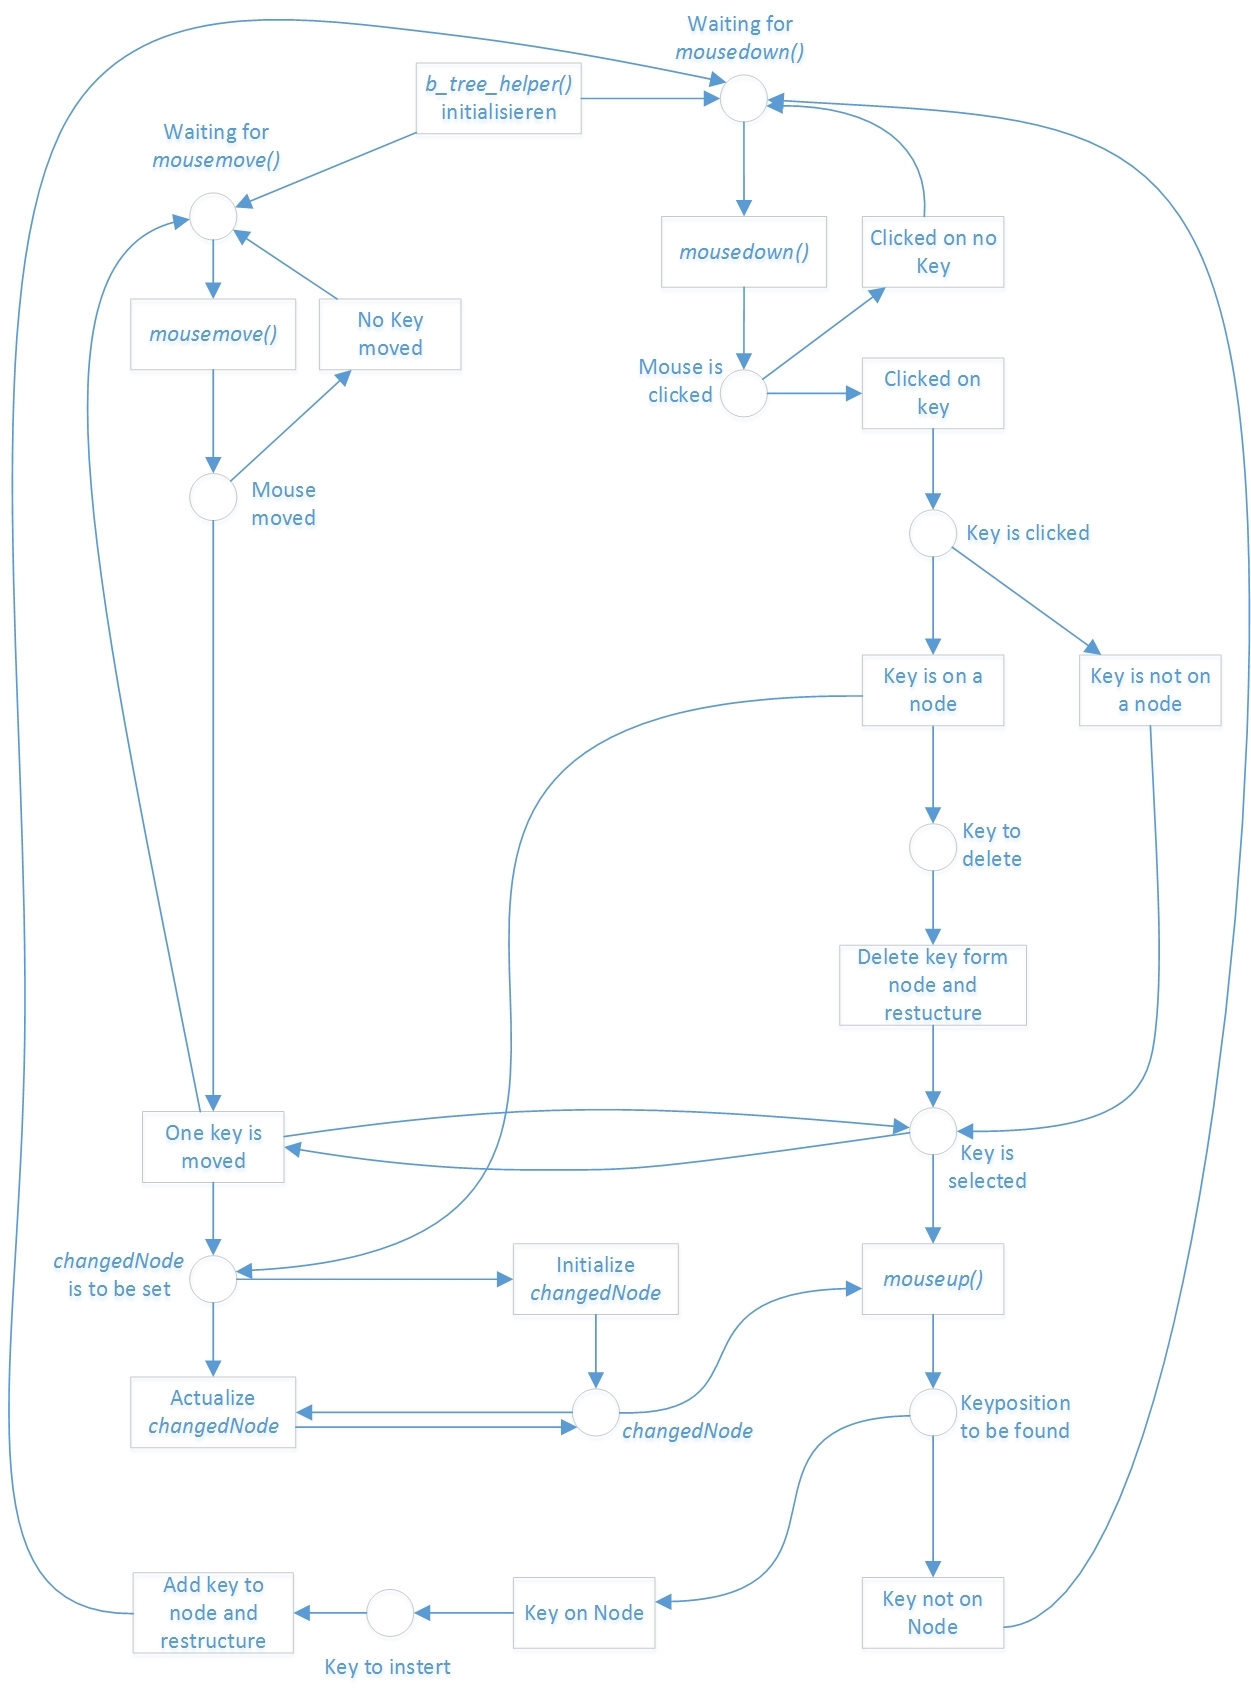
\includegraphics[width=1\textwidth]{graphics/petriNetz.jpg}
  \caption{Petri-Netz des Grapheneditors}
  \label{fig:petri}
\end{figure}
Es handelt sich hierbei um die Funktionen \textit{mousemove()} und \textit{mousedown()}. \textit{Mousemove()} schl�gt jedes mal aus, wenn der Mauszeiger �ber den Editor f�hrt. Aus der Stelle \textit{Mouse selected} heraus gibt es zwei m�gliche Folgezust�nde. Wurde kein Schl�ssel bewegt (\textit{No key moved}) wird der n�chste Zustand mit der erneuten Belegung der Stelle \textit{Waiting for mousemove()} erreicht. F�r die Transaktion \textit{One key is moved} muss jedoch die Stelle \textit{Key is selected} belegt sein. F�r die Belegung dieser Stelle muss zuerst die Transaktion \textit{mousedown()} durchlaufen sein. Anschlie�end k�nnen die Transaktionen \textit{Clicked on no key} und \textit{Clicked on Key} ausgef�hrt. Der Grund f�r den direkten R�cksprung zur Stelle \textit{Waiting for mousedown()} �ber die Transaktion \textit{Clicked on no key} erfolgt gegen Ende des Kapitels. Wurde jedoch auf einen Schl�ssel gedr�ckt (\textit{Clicked on key}), wird im  Anschluss die Verzweigung durchlaufen, die zwischen dem Schl�ssel auf (\textit{Key is on node}) oder nicht auf einem Knoten (\textit{Key is not on node}) unterscheidet. Ist der Schl�ssel nicht auf einem Knoten, wird direkt die Stelle \textit{Key is selected} markiert. Ist der Schl�ssel hingegen auf einem Knoten wird zuerst die Stelle \textit{changeNode is to be set} markiert. W�hrenddessen wird die Transaktion \textit{Delete key from node and restructure} durchlaufen, sodass die Stelle \textit{Key is selected} schlie�lich auch �ber diese Verzweigung markiert wurde.


In folgenden Absatz wird das Teilnetz um die Stellen \textit{changedNode is to be set} und \textit{changedNode} vorgestellt. Bei \textit{changedNode} handelt es sich um eine Variable, die den zuletzt ge�nderten Schl�ssel beinhaltet. Enth�lt diese Variable einen Wert, dann ist die gleichnamige Stelle im Petri-Netz markiert. Um die Stelle zu markieren k�nnen zwei Transaktionen durchlaufen werden. Zum einen gibt es die Transaktion \textit{Initialize changedNode}, zum anderen \textit{Actualize changedNode}, wobei bei dieser \textit{changedNode} bereits markiert sein muss. Die f�r beide Transaktionen ausgehende Stelle ist \textit{changedNode is to be set}. Die zur Markierung dieser Stelle notwendigen Transaktionen sind \textit{One key is moved} und \textit{Key is on a node}. Dies bedeutet, dass die Variabel \textit{changeNode} gesetzt wird, sobald ein Schl�ssel, der auf einem Knoten liegt, angeklickt, bzw. ausgew�hlt wird. Des weiteren wird die Variable gesetzt, sobald ein ausgew�hlter Knoten -- siehe Abh�ngigkeit zwischen \textit{One key is moved} und \textit{Key is selected} -- auf dem Editor bewegt wird.

Eine von der Stelle \textit{Key is selected} n�chstm�gliche Transaktion ist die Transaktion \textit{mouseup}, welche auf die jQuery-Funktion \textit{mouseup()} referiert. Diese Funktion wird ausgel�st, sobald der Nutzer die Maustaste l�st. Das Petri-Netz zeigt, dass die beiden Stellen \textit{changedNode} und \textit{Key is selected} markiert sein m�ssen, damit die Transaktion \textit{mouseup} durchlaufen werden kann. Insbesondere muss in diesem Fall zwischen der durch die Transaktion \textit{mouseup} repr�sentierten Funktionalit�t und der jQuery-Funkion \textit{mouseup()} differenziert werden. Die jQuery-Funktion \textit{mouseup()} wird ausgel�st, sobald der Nutzer die Maustaste l�st, folglich auch, wenn kein Schl�ssel ausgew�hlt ist. Der auftretende Widerspruch, der durch die Forderung des Petri-Netz nach einen gew�hlten Knoten f�r die Ausf�hrung der Transaktion auftritt, wird  durch Betrachtung der in der Funktion \textit{mouseup()} steckenden, durch die Transaktion beschriebenen, Funktionalit�t aufgel�st. Die durch die Transaktion \textit{mouseup} beschriebene Funktionalit�t enth�lt die notwendige Bedingung, dass ein ver�nderter Schl�ssel vorhanden sein muss. Wird diese Bedingung nicht erf�llt, wird die Funktion abgebrochen. Auf Basis dieser Argumentation ist die durch die Transaktion \textit{mouseup} beschriebene Funktionalit�t nur mit dem Vorhandensein einer \textit{changedNode} verf�gbar, obwohl die jQuery-Funktion \textit{mousemove()} ausgel�st worden ist. Hiermit ist ebenso das Enden der Transaktion \textit{Clicked on no Key} in der Stelle \textit{Waiting for mousedown()} begr�ndet. Hiernach wird nach dem l�sen der Maustaste zwar die jQuery-Funktion \textit{mouseup()} ausgel�st, die aus der Funktion resultierende Funktionalit�t wird jedoch nicht angesprochen.




\subsubsection{Implementierungsdetails}
\label{sec:editorImplemenierungsdetails}

In diesem Kapitel wird die Umsetzung der in Kapitel \ref{sec:editorFunktionalitaet} beschriebene Funktionalit�t der Echtzeitverarbeitung des Grapheneditors vorgestellt. Hierf�r wird zuerst auf die wichtigen Datenstrukturen eingegangen. Anschlie�end werden die f�r die Gesamtfunktionalit�t wichtigen Teilfunktionalit�ten veranschaulicht. Zu diesem Zweck wird insbesondere auf die bereits in Kapitel \ref{sec:editorFunktionalitaet} vorgestellten Teilfunktionalit�ten eingegangen.

Die zentrale Datenstruktur f�r die Echtzeitverarbeitung der Schl�sselausrichtung liefert das mehrdimensionales Array \pfile{nodesPerTier}. Der Datenstruktur kann man die Knoten einer Schicht entnehmen, wobei die einzelnen Knoten wiederum �ber ihre jeweiligen Schl�ssel verf�gen. Alle Knoten einer Schicht meint in diesem Zusammenhang alle Knoten einer bestimmten H�he. So verwaltet die h�chste Arraydimension die Schichten des B-Baums. Insgesamt ist der mehrdimensionale Array so aufgebaut, dass die oberste Schicht des B-Baums auf Position null in dem Array der obersten Dimension abgebildet wird. Die zweite Dimension des Arrays beinhaltet die Knoten einer Schicht. Das Arrays auf Position Null beinhaltet diesbez�glich den Wurzelknoten. Auf Position Eins beinhaltet der Array der ersten Dimension die n�chste Schicht, sodass dort ein Array mit den Kindsknoten der Wurzel  abgelegt ist. Die weiteren Positionen enthalten demnach folglich die weiteren Schichten. 
Die einzelnen Knoten werden wiederum auch durch Arrays dargestellt, welche alle Schl�ssel eines Knotens enthalten. Somit handelt es sich bei dem Array \pfile{nodesPerTier} um ein dreidimensionales Array mit Schichten auf der ersten, Knoten auf der zweiten und Schl�sseln auf der dritten Dimension. 

Eine weitere wichtige Datenstruktur ist das Array \pfile{nodeListBounds}. Diese Datenstruktur enth�lt die Grenzen, in denen ein Schl�ssel als Schl�ssel innerhalb eines Knotens erkannt wird. Wird folglich ein Sch�ssel auf dem Editor innerhalb dieser Grenzen abgelegt, wird ein Positionierungsprozess angesto�en, in dem die Schl�ssel eines Knotens neu positioniert werden. Das Array \pfile{nodeListBounds} ist dem Array \pfile{nodesPerTier} stark nachempfunden. So handelt es sich ebenfalls um ein dreidimensionales Array, wobei auch hier die Schichten auf der ersten und die Knoten auf der zweiten Dimension abgelegt werden. In der dritten Dimension sind jedoch anstatt von Schl�sseln die Grenzen der einzelnen Knoten gespeichert. 


Die Funktion \pfile{b\_tree\_helper} ist die Hilfsfunktion, welche eine Echtzeitverarbeitung der Nutzereingabe erm�glicht. Sie bekommt als Parameter die beiden Graphen, den Vordergrund- und den Hintergrundgraphen, und die Ordnung \textit{t} �bergeben.


\subsubsection{Aufbau des B-Baums im Hintergrund}
\label{sec:aufbauBBaumHintergrund}
Dieser Abschnitt erl�utert das Prinzip nach dem die B-Baum-Struktur im Hintergrund des Grapheneditors aufgebaut wird. 


 \bibliography{Bachelorarbeit}
  \bibliographystyle{alpha}
 

  \diplomabschlusserklaerung{(Abgabedatum)}
\end{document}
